\documentclass{article}
\usepackage{amsmath}
\usepackage{esint}
\usepackage[utf8]{inputenc}
\usepackage{listings}
\usepackage{graphicx}
\usepackage{float}
\graphicspath{{/home/david/Documents/}}
\lstset{frame=single}
\linespread{1.5}
\usepackage[dvipsnames]{xcolor}
\usepackage{hyperref}



\begin{document}
	\title{INF 1400 - Oppsummering}
	\author{Dawid Kuleczko}
	\maketitle	
	\tableofcontents
	
	\section{Digital representasjon og binær logikk:}
	\subsection{Tallsystemer:}
	
	I dette kurset skal vi legge spesielt vekt på binære tall, men heksadesimale tall og octale tall, samt tall fra andre tallsystemer, kan også forekomme.
	
	Til daglig bruker vi desimal, altså 10-tallsystemet. Et desimalt tall er representert ved symbolene fra 0 til 9.
	
	eks. $(951)_{dec} = 9 \cdot 10^2 + 5 \cdot 10^1 + 1 \cdot 10^0$
	
	Et binært tall er representert ved symbolene 
	0 og 1.
	
	eks. $ (101)_{bin} = 1 \cdot 2^2 + 0 \cdot 2^1 + 1 \cdot 2^0$
	
	Et heksadesimalt tall er representert ved symbolene 
	fra 0 til F der tallene etter 9 er:
	10 = A
	11 = B
	12 = C
	13 = D
	14 = E
	15 = F
	
	eks. $(5BF)_{hex} = 5 \cdot 16^2 + 11 \cdot 16^1 + 15 \cdot 16^0$ 
	
	Et oktalt tall er representert ved symbolene fra 0 til 8.
	
	eks. $(853)_{oct} = 8 \cdot 8^2 + 5 \cdot 8^1 + 3 \cdot 3^0$

	\subsection{Konvertering:}
	
	\subsubsection{Konvertering fra grunntall r til desimaltall:}
	Generelt:
	$(...a_2 a_1 a_0 , a_{-1} a_{-2}...) = ... + a_2 \cdot r^2 + a_1 \cdot r^1 + a_0 \cdot r^0 , a_{-1} \cdot r^{-1} a_{-2} \cdot r^{-2} + ..$
	
	eks.
	$(1A5,1C)_{16} = 1 \cdot 16^2 + A \cdot 16^1 + 5 \cdot 16^0 + 1 \cdot 16^{-1} + 12 \cdot 16^{-2} = (421,109375)_{10}$
	
	
	
	\subsubsection{Konvertering av desimal til binær:}
	
	Eks. $(23)_{10}$
	$$ 23/2 = 11 + 1/2 \qquad a_0 = 1 $$
	$$ 11/2 = 5 + 1/2 \qquad a_1 = 1 $$
	$$ 5/2 = 2 + 1/2 \qquad a_2 = 1 $$	
	$$ 2/2 = 1 + 0/2 \qquad a_3 = 0 
	$$
	$$1/2 = 0 + 1/2 \qquad a_4 = 1
	$$
	
	Vi leser det binære tallet nedfra $(10111)_{2}$
	
	\subsubsection{Konvertering av kommatall i desimal til binær :}
	Eks. $(0.3125)_{10}$
	$$ 0.3125*2 = 0.625 \qquad a_{-1} = 0 $$
	$$ 0.625*2 = 1.25 \qquad a_{-2} = 1 $$
	$$ 0.25*2 = 0.5 \qquad a_{-3} = 0 $$	
	$$ 0.5*2 = 1.0 \qquad a_{-4} = 1 $$
		
	Vi leser det binære tallet oppfra $(0.0101)_{2}$
	
	\subsubsection{Konvertering fra desimal til grunntall “r”:}
	Samme måte som over bare med "r" isteden for 2.
	
	Eks. $(12)_{10}$ til 3-tallsystemet:
	
	$$ 12/3 = 4 + 0/3 \qquad a_0 = 0$$
	$$ 4/3 = 1 + 1/3 \qquad a_1 = 1$$
	$$ 1/3 = 0 + 1/3 \qquad a_2 = 1 $$
	
	Tallet blir da $(110)_3$ i 3 tallsystemet.
	
	\subsection{Logiske porter:}
		
	\begin{figure}[H]
		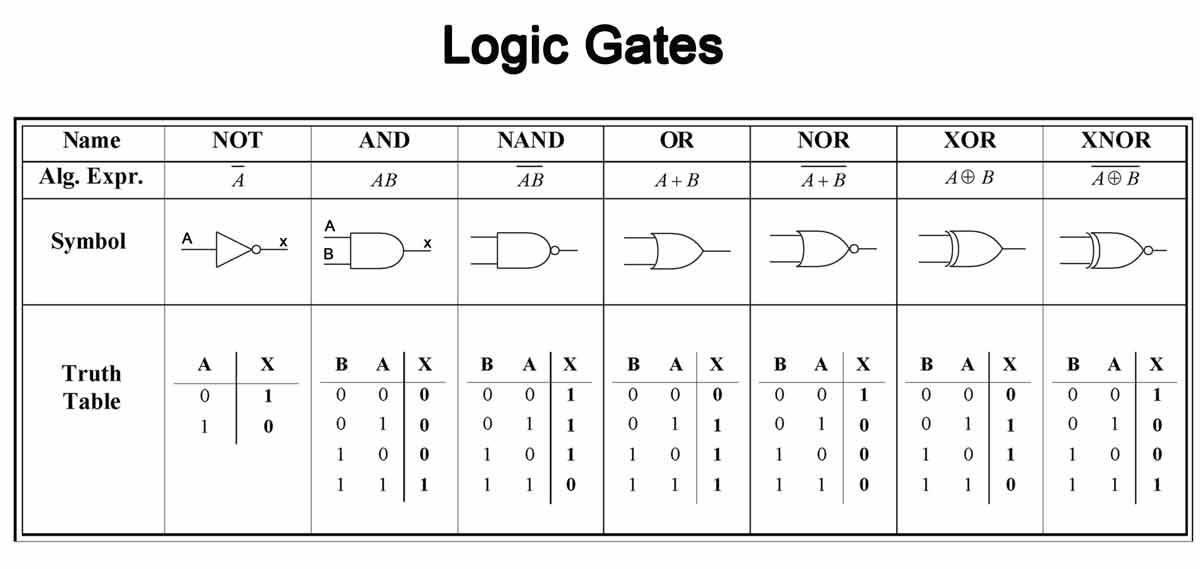
\includegraphics[scale=0.35]{GATES.jpg}
		\caption{Logiske porter}
	\end{figure}
	
	\begin{figure}[H]
		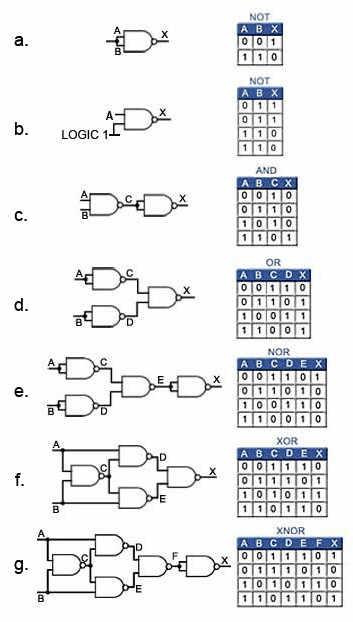
\includegraphics{NAND.jpg}
		\caption{Logiske porter som 2 inputs NAND-porter}
	\end{figure}
	
		
	\begin{figure}[H]
		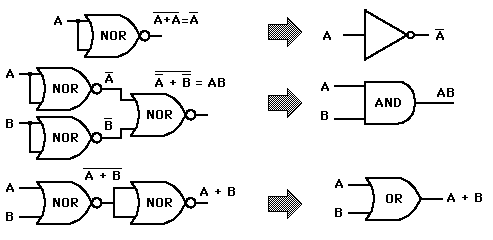
\includegraphics[scale=0.6]{nor.png}
		\caption{Logiske porter som NOR-porter}
	\end{figure}
	
	\begin{figure}[H]
		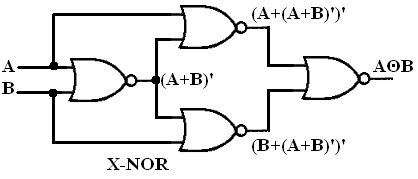
\includegraphics[scale=0.6]{NasX.PNG}
		\caption{XNOR laget av NOR-porter}
	\end{figure}
	
	
	\subsection{Huntington's postulater}
	\begin{figure}[H]
		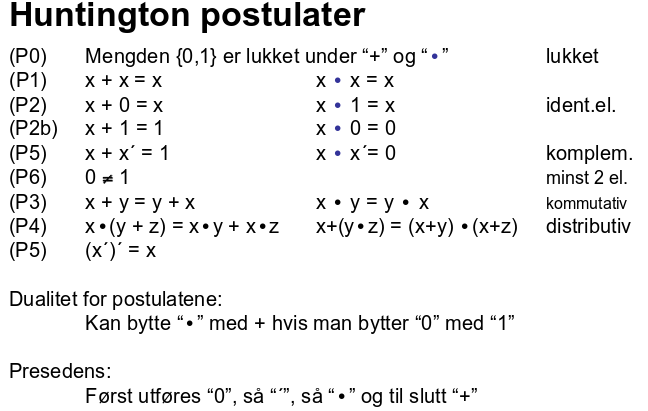
\includegraphics[scale=0.35]{Huntington.png}
		\caption{Huntington's postulater}
	\end{figure}
	
	
	\section{Boolsk algebra:}
	
	\begin{figure}[H]
		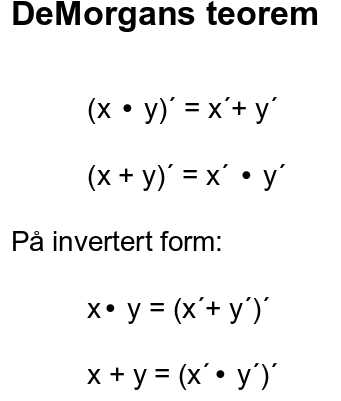
\includegraphics[scale=0.4]{DeMorgan.png}
		\caption{DeMorgans teorem}
	\end{figure}
	
	\begin{figure}[H]
		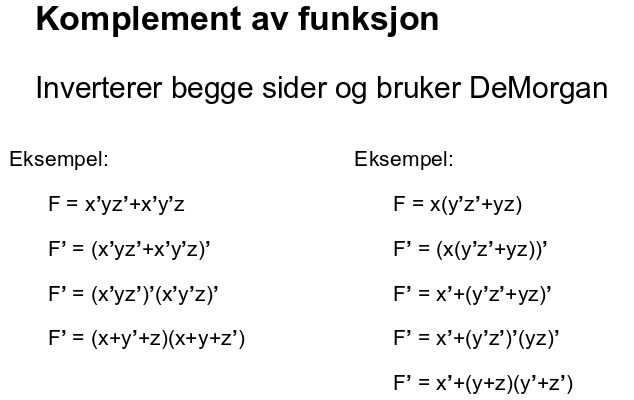
\includegraphics[scale=0.55]{Komplement.png}
		\caption{Komplement av funkson}
	\end{figure}
	
	\begin{figure}[H]
		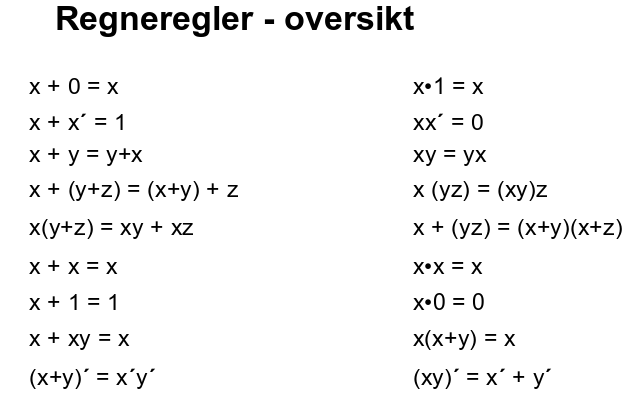
\includegraphics[scale=0.6]{Regneregler.png}
		\caption{Regne regler for boolsk algebra}
	\end{figure}
	
	\subsection{Boolske funksjoner med sannhetstabell}
	En boolsk funksjon kan visualiseres i en 
	sannhetstabell.
	En gitt	funksjon har kun en	sannhetstabell 
	Men, en gitt sannhetstabell har uendelig mange funksjonsuttrykk.
	
	\textbf{Eksempel: F = x + y' z}
	
		\begin{center}
			\begin{tabular}{|c|c|}
				\hline
				XYZ & F \\ \hline
				000 & 0  \\ \hline
				001 & 1  \\ \hline 
				010 & 0  \\ \hline
				011 & 0  \\ \hline 
				100 & 1  \\ \hline
				101 & 1  \\ \hline
				110 & 1  \\ \hline
				111 & 1  \\ \hline
				
			\end{tabular}
		\end{center}
	
	
	\subsection{Forenkling av uttryk}
	En funksjon kan forenkles ved regneregler for å gjøre den lettere å håndere og implementere.
	
	\begin{figure}[H]
		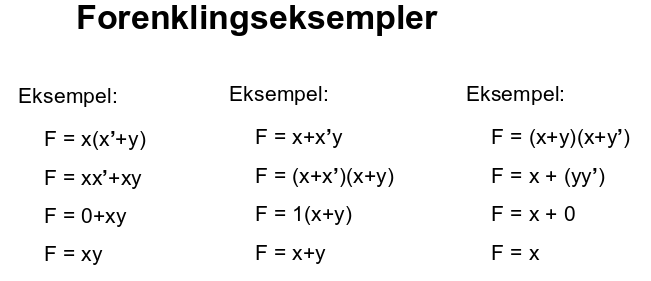
\includegraphics[scale=0.6]{Forenkling.png}
		\caption{Forenklingseksempler av noen funksjoner}
	\end{figure}
	
	\begin{figure}[H]
		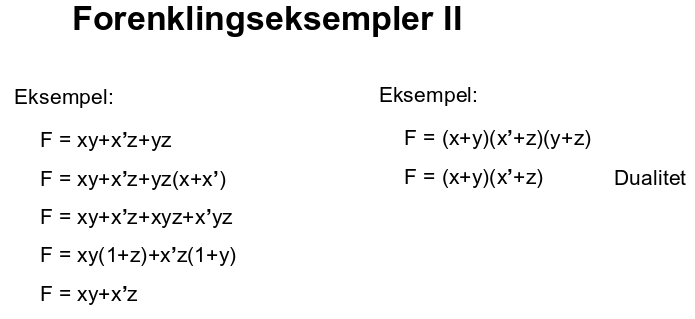
\includegraphics[scale=0.6]{Forenkling2.png}
		\caption{Forenklingseksempler av noen funksjoner}
	\end{figure}
	
	\subsection{Maksterm/Minterm}
	
	\begin{figure}[H]
		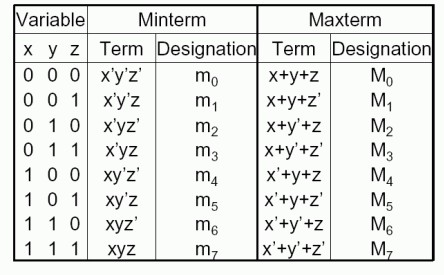
\includegraphics[scale=0.8]{maksmin.jpg}
		\caption{Tabell for minterm og maksterm}
	\end{figure}
	
	Mintermer har notasjon $m_x$
	
	$F\textcolor{Violet}{(x,y,z)} = \sum\textcolor{Violet}{(m_3, m_6)} = \sum\textcolor{Violet}{(3, 6)} = \textcolor{Violet}{ x'yz + xyz'} $
	
	Makstermer har notasjon $M_x$
	
	$F\textcolor{Violet}{(x,y,z)} = \Pi \textcolor{Violet}{(M_3, M_6)} = \Pi \textcolor{Violet}{(3, 6)} = \textcolor{Violet}{(x+y'+z')(x'+y'+z)} $
	
	\subsubsection{Minterm:}
	I en funksjon kan en binær variabel x opptre som x eller x'.	En funksjon kan være gitt på “sum av produkt” form.
	Eksempel: F = xy + xy' + x
	
	Hvert “produktledd” som inneholder alle variablene kalles en minterm. For to variable finnes det 4 forskjellige mintermer: xy + xy' + x'y + x'y'
	For 3 variable finnes det $2^3$ forskjellige mintermer. 
	
	Hvis man generer en funksjon ut i fra sannhetstabellen får man en sum av mintermer
	
	Eksempel:  F = \textcolor{Aquamarine}{x'y'z} + \textcolor{BurntOrange}{xy'z'} + \textcolor{WildStrawberry}{xyz'}
	
	
	\begin{center}
		\begin{tabular}{|c|c|}
			\hline
			XYZ & F \\ \hline
			000 & 0  \\ \hline
			001 & \color{Aquamarine}1  \\ \hline 
			010 & 0  \\ \hline
			011 & 0  \\ \hline 
			100 & \color{BurntOrange}1  \\ \hline
			101 & 0  \\ \hline
			110 & \color{WildStrawberry}1  \\ \hline
			111 & 0  \\ \hline
			
		\end{tabular}
	\end{center}
	
	En sannhetstabell kan sees på som en liste av mintermer.
	
	\subsubsection{Maksterm:}
	
	En funksjon kan være gitt på “produkt av sum” form.
	
	Eksempel: F = (x+y)(x+y')y 
	Hvert "summeledd" som inneholder alle variablene kalles maksterm.
	
	For to variable finnes det 4 forskjellige makstermer:
	(x'y)(x+y')(x'+y)(x'+y')
	
	For n variable finnes det $2^n$ forskjellige makstermer.
	
	\subsection{Designprosedyre }
	
	Det er ikke alltid at det enkleste funksjonsuttrykket resulterer i den enkleste port-implementasjonen.
	
	Ved forenkling på portnivå må man vite hvilke porter man har til rådighet, og så justere funksjonsuttrykket mot dette. (håndverk) 
	
	\textbf{Generell design	prosedyre}
	
	1.Bestem hvilke signal som er innganger og 
	utganger
	
	2.Sett opp sannhetstabell for alle 
	inngangskombinasjoner
	
	3.Generer funksjonsuttrykket som sum av 
	mintermer 
	
	4.Tilpass / forenkle funksjonsuttrykket mot 
	aktuelle porter 
	
	\section{Karnaugh diagram:}
	Grafisk metode for forenkling av Boolske uttryk
	\begin{figure}[H]
		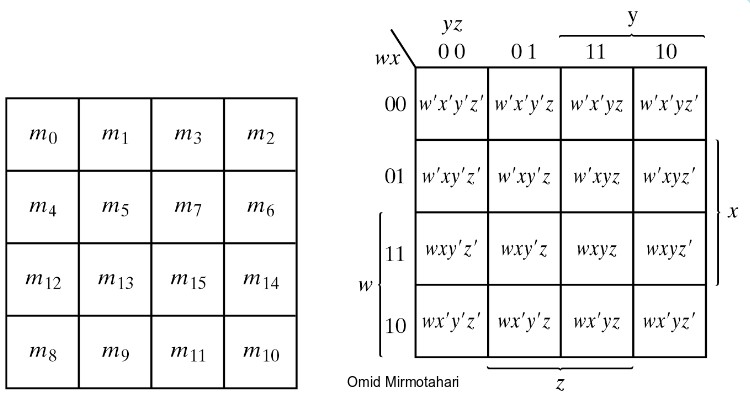
\includegraphics[scale = 0.6]{KarnaD.jpg}
		\caption{Karnaugh diagram med mintermene}
	\end{figure}
	
	\begin{figure}[H]
		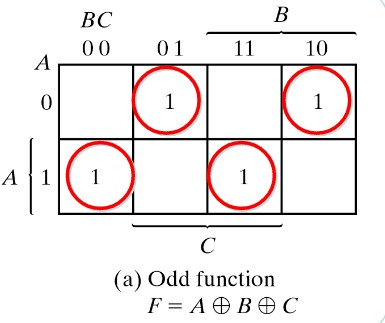
\includegraphics[scale = 0.6]{XOR.jpg}
		\caption{XOR}
	\end{figure}
	
	\begin{figure}[H]
		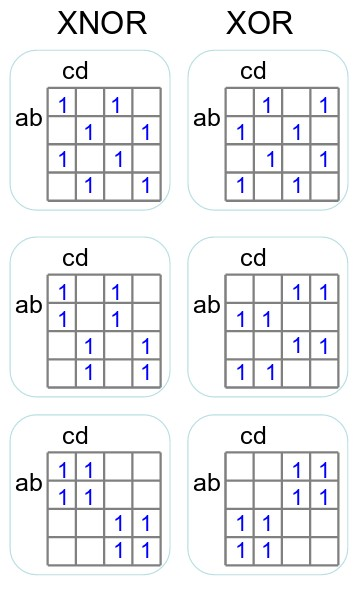
\includegraphics[scale = 0.7]{X.jpg}
		\caption{XNOR og XOR}
	\end{figure}
	
	\begin{figure}[H]
		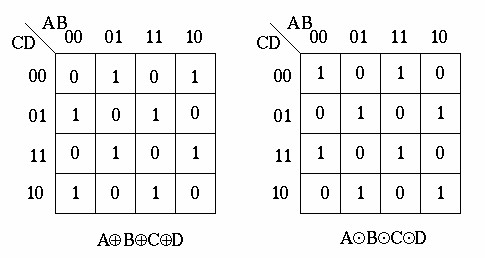
\includegraphics[scale = 0.7]{x.jpg}
		\caption{XNOR og XOR}
	\end{figure}
	
	
	\section{Kobinatorisk logikk:}
	
	\subsection{Binær addisjon:}
	 Prosedyren for binær addisjon er identisk med prosedyren for desimal addisjon:
	 
	 Eks: 
	 $\begin{bmatrix}
	 0 1 0 1 \\
	 1 0 1 1 & + \\
	 ------- \\
	 1 0 0 0 0
	 \end{bmatrix}$
	5 + 11 = 16
	\subsection{Binær substraksjon:}
	\begin{figure}[H]
		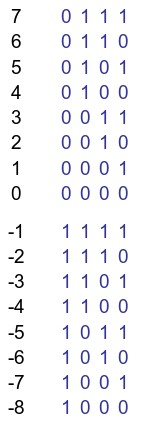
\includegraphics[scale = 0.7]{Nega.jpg}
		\caption{Representasjon av binære negative tall}
	\end{figure}
	
	For å substrahere negative binære tall, bruker man toerkomplement metoden.
	
	Det tallet som skal substraherers med må inverteres og plusses på 1, deretter skal det plusses med den andre tallet. Tallet til overs går ut.
	
	Eks: 
	$\begin{bmatrix}
	1 1 0 1 \\
	1 0 1 1 & -\\
	------- \\
	\end{bmatrix}$ 
	$\begin{bmatrix}
	1 1 0 1 \\
	0 1 0 1 & +\\
	------- \\
	(1) 0 0 1 0
	\end{bmatrix}$
	13-11 = 2
	
	13+5=18 = 1 0 0 1 0
	
	\subsection{Binære addere:}
	\subsubsection{Halvadder:}
	Halvaddere tar ikke mente inn.
	
	Halvadder implementasjon
	\begin{figure}[H]
		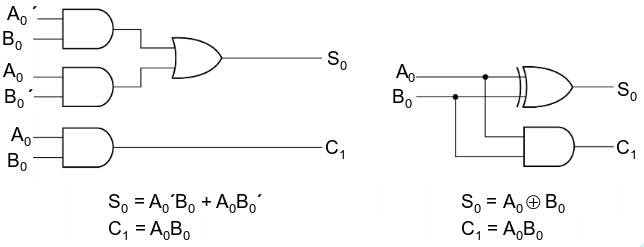
\includegraphics[scale = 0.7]{halvadd.jpg}
		\caption{Halvadder implementasjon}
	\end{figure}
	
	\subsubsection{Fulladder:}
	Fulladder tar mente inn.
	
	Fulladder implementasjon
	\begin{figure}[H]
		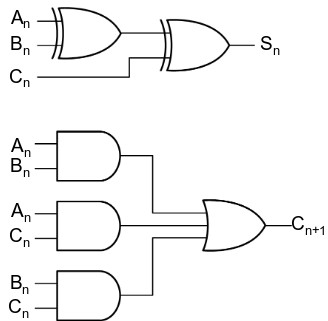
\includegraphics[scale = 0.7]{Fulladd.jpg}
		\caption{Fulladder implementasjon}
	\end{figure}
	
	\subsubsection{Et adder system}
	\begin{figure}[H]
		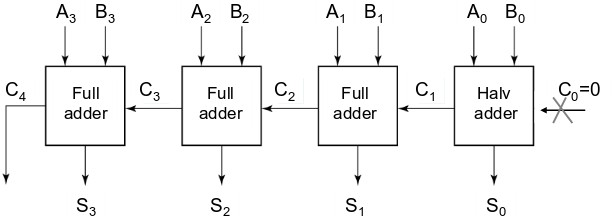
\includegraphics[scale = 0.6]{adderment.jpg}
		\caption{Et system av halv og fulladdere}
	\end{figure}
	
	\begin{figure}[H]
		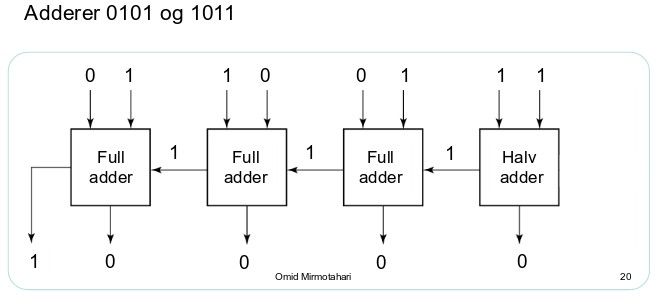
\includegraphics[scale = 0.6]{addeks.jpg}
		\caption{Et eksempel på addisjon av to binære 4-bits tall}
	\end{figure}
	
	\subsection{”Carry Lookahead”}
	 Ønsker å unngå menteforplantning – gir økt hastighet
	 
	 $G_i$ – generate: brukes i menteforplantningen
	 $P_i$ – propagate: påvirker menteforplantningen
	
	\subsection{Komparator:}
	Komparator – sammenligner to tall A og B 
	
	3 utganger: $A=B, A>B\ \text{og} \ A<B$
	
	\begin{figure}[H]
		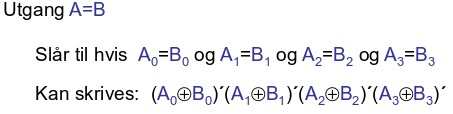
\includegraphics[scale = 0.6]{komp1.jpg}
		\caption{A=B}
	\end{figure}
	
	
	\begin{figure}[H]
		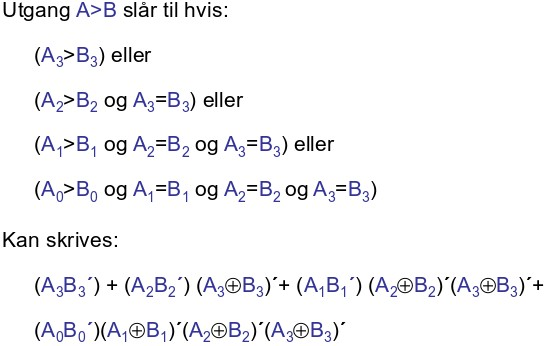
\includegraphics[scale = 0.6]{komp2.jpg}
		\caption{$A>B$}
	\end{figure}
	
	\begin{figure}[H]
		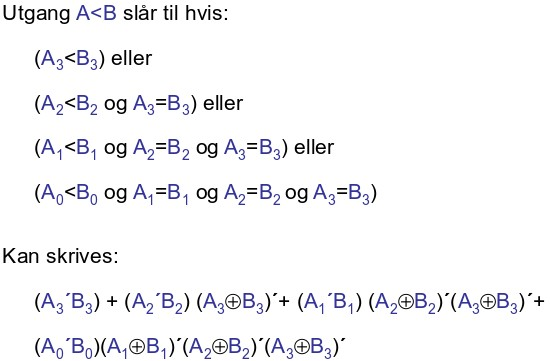
\includegraphics[scale = 0.6]{komp3.jpg}
		\caption{$A<B$}
	\end{figure}
	
	\subsection{Dekoder:}
	 Dekoder – tar inn et binært ord og gir ut alle mintermer. 
	 Kan generere generelle logiske funksjoner direkte fra mintermene på utgangen 
	 Eksempel: 3bit inn/8bit ut 
	 
	\begin{figure}[H]
		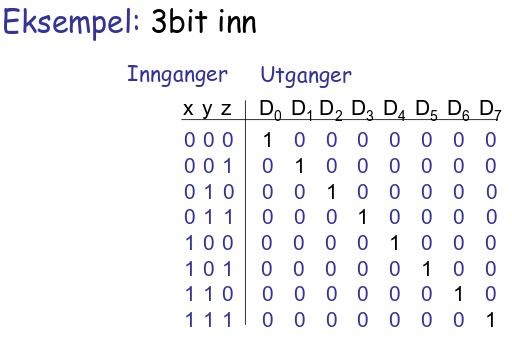
\includegraphics[scale = 0.6]{decoder.jpg}
		\caption{Sannhetstabell til en 3 bits decoder}
	\end{figure}
	
	\subsection{Enkoder:}
	Enkoder er motsatt av dekoder
	
	\begin{figure}[H]
		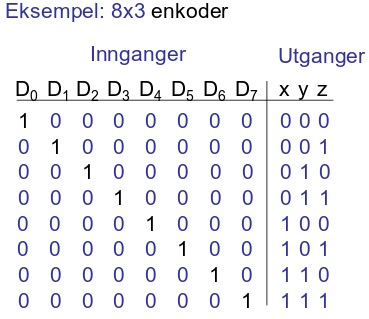
\includegraphics[scale = 0.6]{enkoder.jpg}
		\caption{Sannhetstabell for en 8x3 enkoder}
	\end{figure}
	
	Prioritets-enkoder:
	
	Hvis flere ”1”ere inn - ser kun på inngang med høyst indeks (prioritet) 
	
	
	\subsection{Multiplekser (MUX):}
	Velger hvilke  innganger som slippes ut
	
	\begin{figure}[H]
		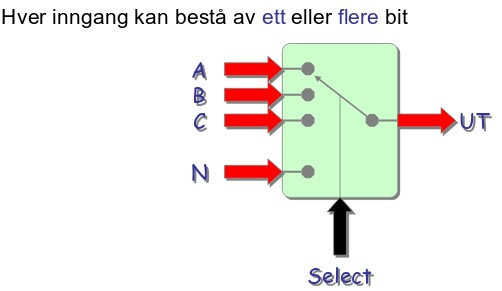
\includegraphics[scale = 0.6]{MUX.jpg}
		\caption{MUX}
	\end{figure}
	
	\begin{figure}[H]
		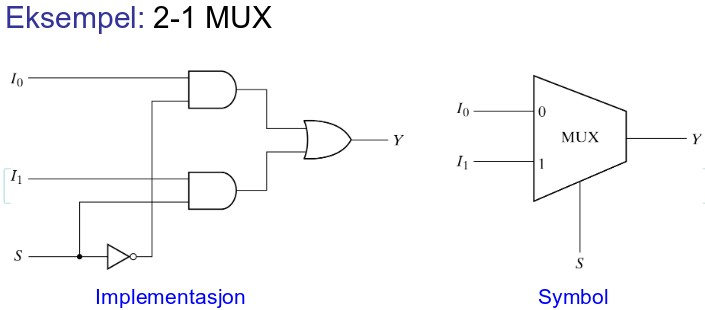
\includegraphics[scale = 0.6]{MUX2.jpg}
		\caption{En 2-1 MUX}
	\end{figure}
	
	
	\subsection{Demulitplekser:}
	Motsatt av MUX, velger hvilke utganger som slippes ut
	
	\begin{figure}[H]
		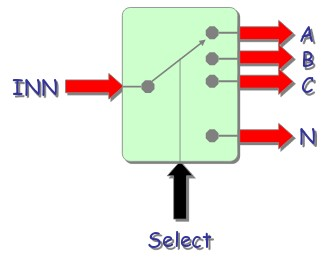
\includegraphics[scale = 0.6]{DEMUX.jpg}
		\caption{Demultiplekser}
	\end{figure}
	
	
	\subsection{Aritmetisk logisk enhet (ALU):}
	En elektronisk krets som utfører aritmetiske og logiske operasjoner	
	
	\section{Sekvensiell logikk:}
	
	Kombinatorisk logikk:
	Utgangsverdiene er entydig gitt av nåværende kombinasjon av inngangsverdier.
	
	Sekvensiell logikk:
	Inneholder hukommelse (låsekretser). Utgangsverdiene er gitt av nåværende kombinasjon av inngangsverdier,  samt sekvensen av tidligere inngangs-­/utgangsverdier.
	
	Mekaniske brytere gir ikke “rene”  logiske nivå ut i
	overgangsfasen.  Slike signaler  må ofte “renses”  ved bruk
	av låsekretser.
	
	I synkrone  sekvensielle kretser skjer endringen(e) i output  samtidig  med endringen i et  klokkesignal. 
	 
	I  asynkrone  sekvensielle kretser skjer endringen(e) i  output  uten  noe  klokkesignal.  
	 
	Nesten alle kretser er synkrone.
	 
	Et klokkesignal er et digitalt signal som veksler mellom 0 og 1 med fast takt. 
	
	\begin{figure}[H]
		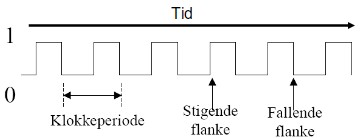
\includegraphics[scale = 0.6]{flanke.jpg}
		\caption{Flanker}
	\end{figure}
	 
	Ønsker så høy klokkefrekvens som mulig, for at hver enkelt operasjon bruker så kort tid som mulig
	 
	Maksimal klokkefrekvens bestemmes av:
	 - Lengde på singalveiene
	 - Last
	 - Forsinkelsene gjennom porter(delay)
	 - Teknologi
	 
	\subsection{Logisk dybde}
	Antall proter et singal passerer fra inngang til utgang, ved å redusere dette minsker forsinkelsen gjennom kretsen.
	
	\begin{figure}[H]
		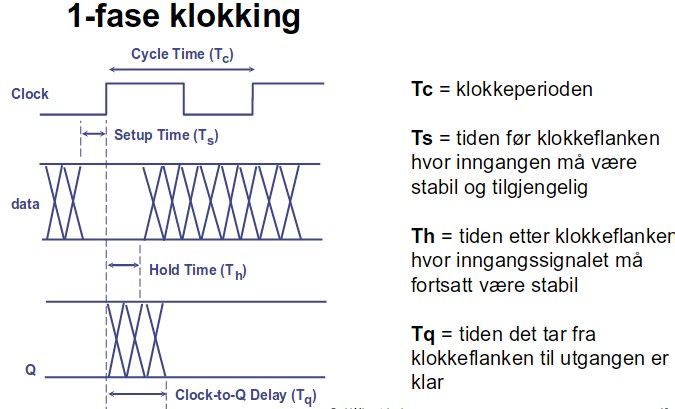
\includegraphics[scale = 0.6]{klokking.jpg}
		\caption{Klokking}
	\end{figure}
	
	\subsection{Latcher(låsekretser):}
	De ulike latchene:
	
	\textbf{SR - Latch}
	
	Set Reset - Latch
	
	Setter Q  til ”1”  hvis den får ”1”  på inngang S. 
	
	Når inngang S går tilbake til ”0” skal Q forbli på ”1”
		
	Kretsen skal resette Q  til ”0”  når den får ”1”  på inngang R.
	
	Når inngang R går tilbake til ”0”  skal Q  forbli på ”0”
	
	Tilstanden ”1”  på både S  og R  brukes	normalt ikke
	
	\begin{figure}[H]
		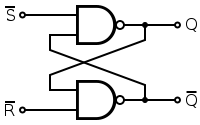
\includegraphics[scale = 0.6]{srlatch.png}
		\caption{SR-Latch med NAND}
	\end{figure}
	
	\begin{figure}[H]
		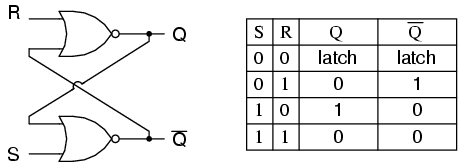
\includegraphics[scale = 0.6]{srL.png}
		\caption{SR-Latch med 2 NOR}
	\end{figure}
	
	\textbf{D - Latch}
	
	Data - Latch
		
	Dataflyten gjennom en  D-­latch  kontrolleres av et  klokkesignal
	
	Slipper  gjennom et  digital  signal  så lenge klokkeinngangen er “1” (transparent)
	
	I  det øyeblikket klokkeinngangen går fra “1”  til “0”  låser utgangen seg på sin nåværende verdi.  
	
	Forandringer på	inngangen vil ikke påvirke utgangsverdien så lenge klokkesignalet er “0”
	
	\begin{figure}[H]
		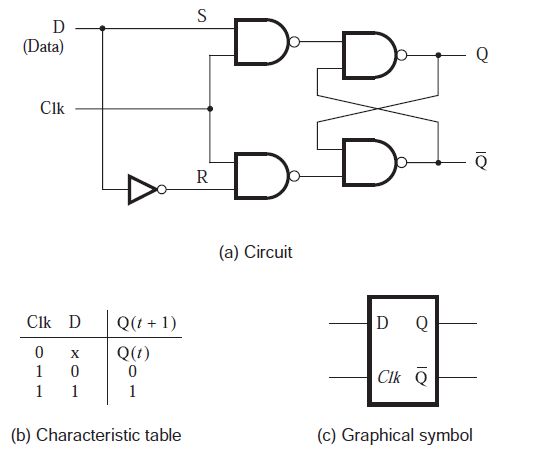
\includegraphics[scale = 0.6]{dL.png}
		\caption{D-Latch}
	\end{figure}
	
	
	\subsection{Flip-Floper:}
	Et 1-bits hukommelseselement som kan	lagre ett bit kalles en flip-flop
	
	En ny verdi kan	bare leses inn og lagres når klokkesignalet går fra 0 til 1 (eller 1 til 0, avhengig av konstruksjonen)
	
	En flip-flop’er har	enten en eller to innganger (pluss klokkesignal) og en utgang
	
	\begin{figure}[H]
		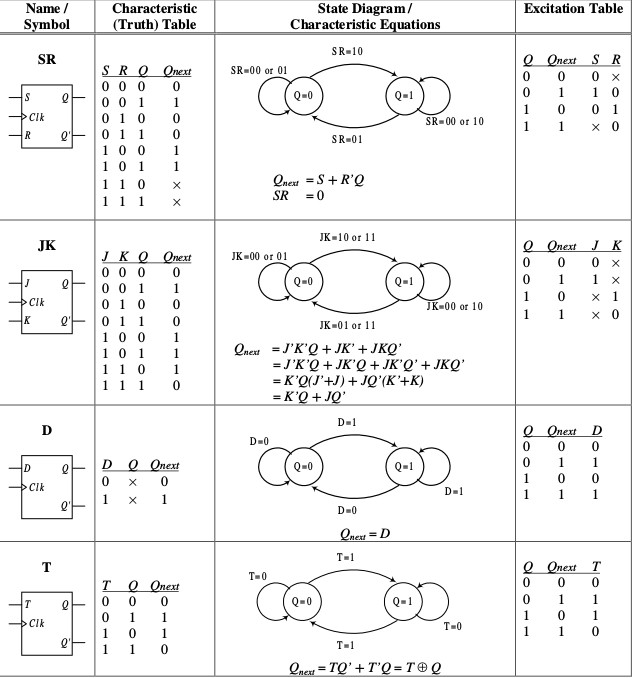
\includegraphics[scale = 0.6]{flip-flop.jpg}
		\caption{Typer Flip-floper}
	\end{figure}
	
	Flip-­Flop’er kommer  i  to  varianter:
	
	• Positiv flanketrigget
	
	• Negativ flanketrigget
	
	På  en  positiv  flanketrigget  Flip-­Flop kan  utgangen  kun  
	skifte  verdi  i  det  øyeblikk  klokkesignalet  går  fra ”0”  til ”1”.
	
	På  en  negativ  flanketrigget  Flip-­Flop  kan  utgangen  
	kun  skifte  verdi  i  det  øyeblikk  klokkesignalet  går  fra
	”1”  til ”0”.
	
	De ulike Flip-Flopene:
	
	\textbf{SR - Flip-flop}
	Set Reset - Flip-Flop
	
	\begin{figure}[H]
		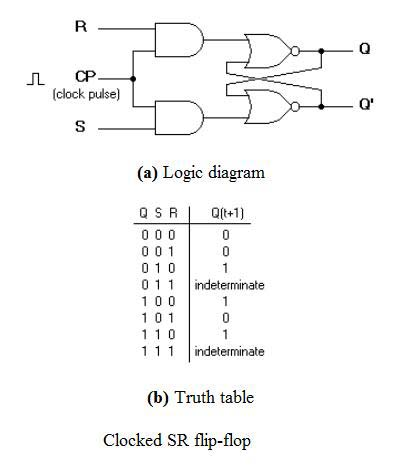
\includegraphics[scale = 0.6]{srFlip.jpg}
		\caption{Kretsoppbygging til en SR-Flip-Flop}
	\end{figure}
	
	\textbf{JK - Flip-flop}
	J(Set) K(Reset) - Flip-Flop
	
	\begin{figure}[H]
		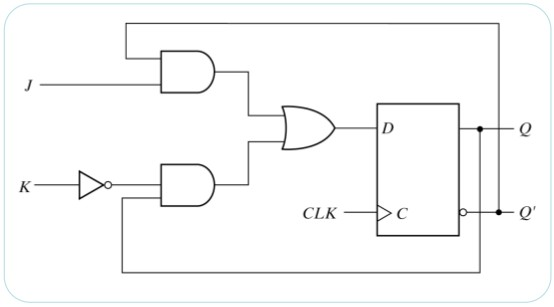
\includegraphics[scale = 0.6]{jkFlip.jpg}
		\caption{Kretsoppbygging til en JK-Flip-Flop}
	\end{figure}
	
	\begin{figure}[H]
		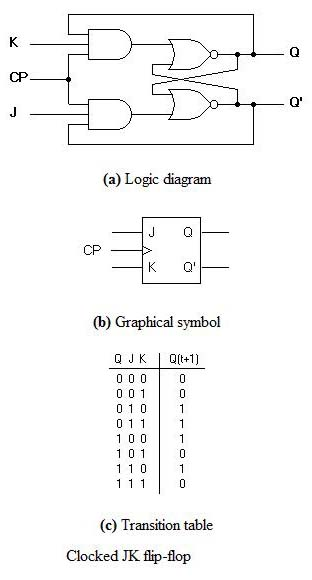
\includegraphics[scale = 0.6]{jkFlip2.jpg}
		\caption{Typer Flip-floper}
	\end{figure}
	
	\textbf{D - Flip-flop}
	Data - Flip-Flop
	
	\begin{figure}[H]
		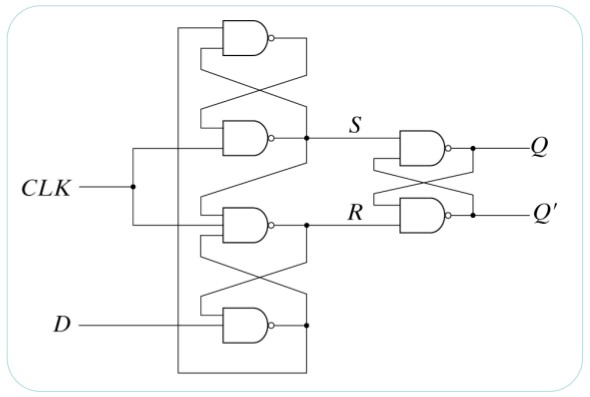
\includegraphics[scale = 0.6]{dFlip.jpg}
		\caption{Kretsoppbygning til en D-Flip-Flop}
	\end{figure}
	
	\begin{figure}[H]
		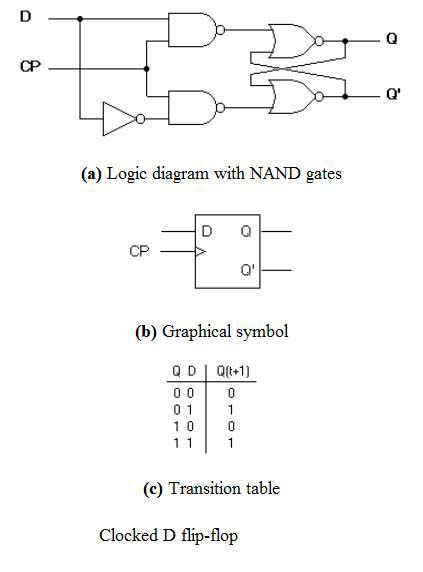
\includegraphics[scale = 0.6]{dFlip2.jpg}
		\caption{Kretsoppbygning til en D-Flip-Flop}
	\end{figure}
	
	\textbf{T - Flip-flop}
	Toggle - Flip-Flop
	
	\begin{figure}[H]
		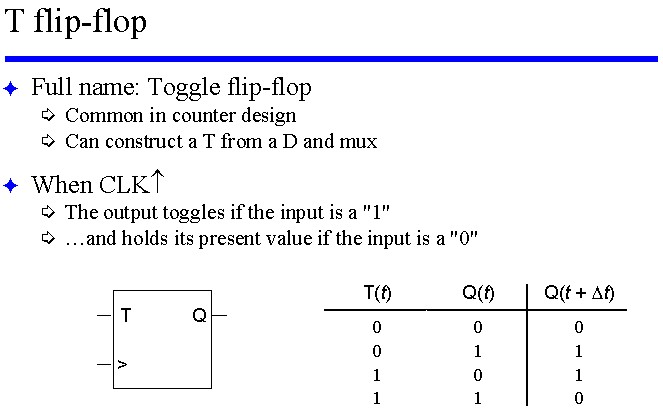
\includegraphics[scale = 0.6]{tFlip.jpg}
		\caption{T - Flip-Flop}
	\end{figure}
	
	\begin{figure}[H]
		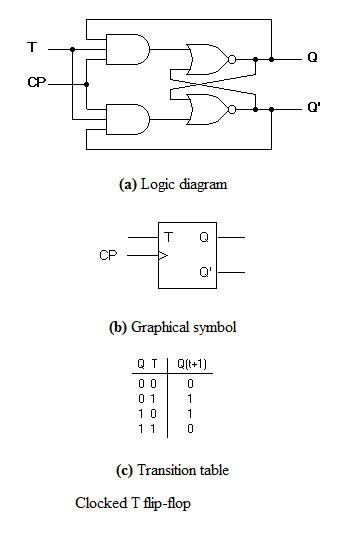
\includegraphics[scale = 0.6]{tFlip2.jpg}
		\caption{T - Flip-Flop}
	\end{figure}
	
	
	\section{Tilstandsmaskiner:}
	Tilstandsmaskiner er en metode til å beskrive systemer med logisk og dynamisk (tidsmessig) oppførsel. 
	
	En tilstandsmaskin er et sekvensielt system som gjennomløper et sett med tilstander styrt av verdiene på inngangssignalene 
	
	Brukes mye innen: 
	
	–Logiske/digitale styresystemer 
	
	–Sanntidssystemer 
	
	–Telekommunikasjon 
	
	–Kompilatorteknikk 
	
	–Digitalteknikk 
	
	Modellen av en tilstandsmaskin:
	
	-Tilstander
	
	er et begrep som benyttes til å beskrive systemets tilstand. 
	 
	er et verdisett/attributter som beskriver systemets egenskaper
	
	- Hendelser
	
	endrer systemet fra en tilstand til en annen
	
	er et begrep som benyttes om innganger/påvirkninger på 
	systemet 

	kan beskrives som en plutselig og kortvarig påvirkning av 
	systemet. 
	
	- Aksjoner
	
	er det som kommer ut av systemet(resultatet)
	er en respons på en hendelse 

	
	\subsection{Tilstandstabell}
	Sannhetstabell for tilstandsmaskiner
	
	
	\begin{figure}[H]
		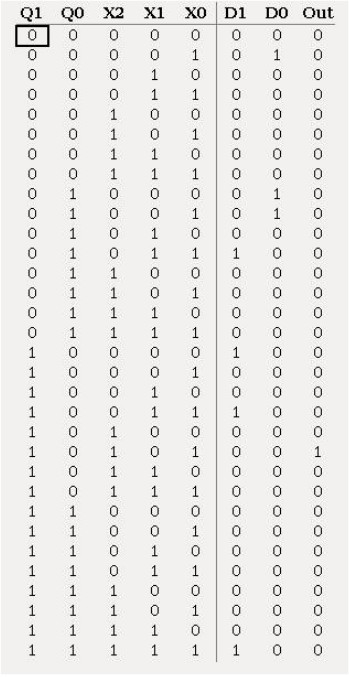
\includegraphics[scale = 0.6]{ekstil.jpg}
		\caption{Eksempel på en tilstandstabell fra oblig 2}
	\end{figure}
	
	\subsection{Tilstandsdiagram}
	
	For å visualisere oppførselen til systemer brukes gjerne tilstandsdiagramer
	
	\begin{figure}[H]
		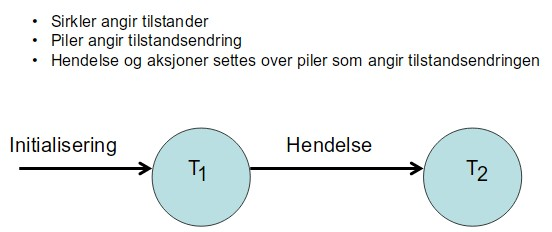
\includegraphics[scale = 0.6]{tilstanddiagram.jpg}
		\caption{Tilstandsdiagram}
	\end{figure}
	
	\begin{figure}[H]
		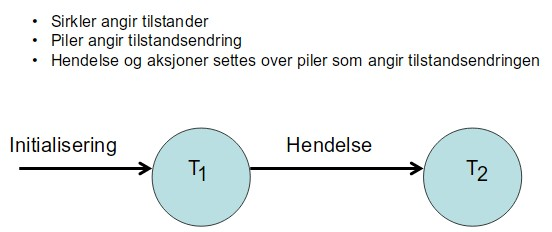
\includegraphics[scale = 0.6]{tilstanddiagram.jpg}
		\caption{Tilstandsdiagram}
	\end{figure}
	
	\begin{figure}[H]
		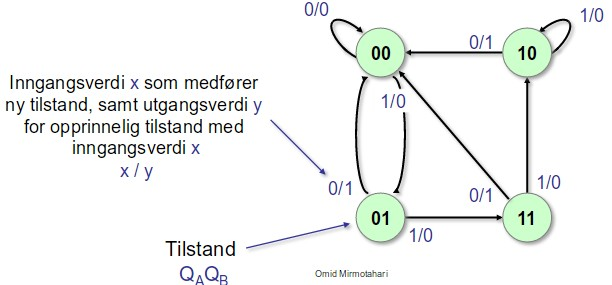
\includegraphics[scale = 0.6]{tilstandeks.jpg}
		\caption{Eksempel på en tilstandsdiagram}
	\end{figure}
	
	\subsection{Reduksjon av antall tilstander}
	 Hvis to tilstander har samme utgangssignal, samt leder til de samme nye tilstandene gitt like inngangsverdier,
	 er de to opprinnelige tilstandene like. En tilstand som er lik en annen tilstand kan fjernes
	 
	 Eksempel:
	 \begin{figure}[H]
	 	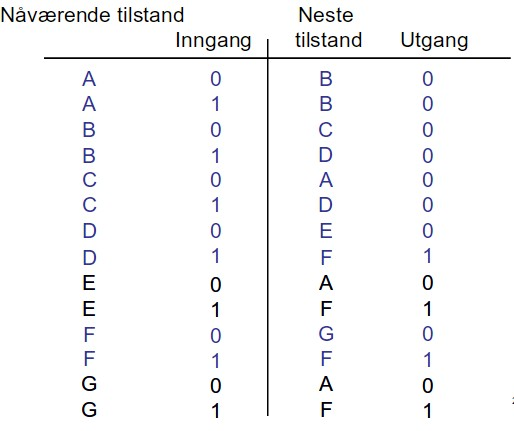
\includegraphics[scale = 0.6]{red.jpg}
	 	\caption{Eksempel på reduksjon av tilstander}
	 \end{figure}
	 
	 Vi ser at tilstand G er lik E
	 
	 Vi kan fjerne tilstand G og erstatte hopp til G med hopp til E
	 
	 Etter det ser vi at tilstand F blir lik D, da fjerner vi F
	 
	 Slik kan vi redusere tilstandene.
	 
	 	
	\subsection{Tilordning av tilstandskoder}
	\begin{figure}[H]
		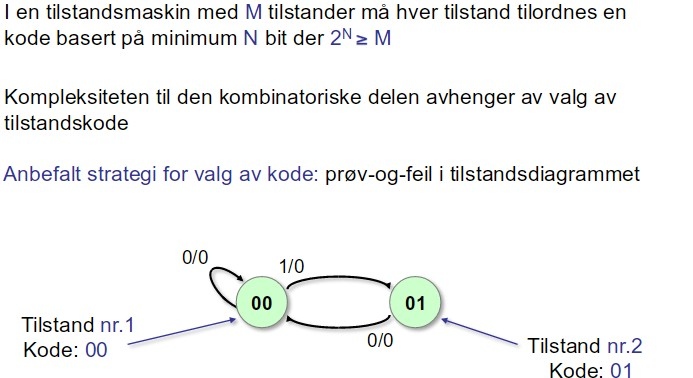
\includegraphics[scale = 0.6]{tilordning.jpg}
		\caption{Tilordning av tilstandskoder}
	\end{figure}
	
	\subsection{Ubrukte tilstander}
	\begin{figure}[H]
		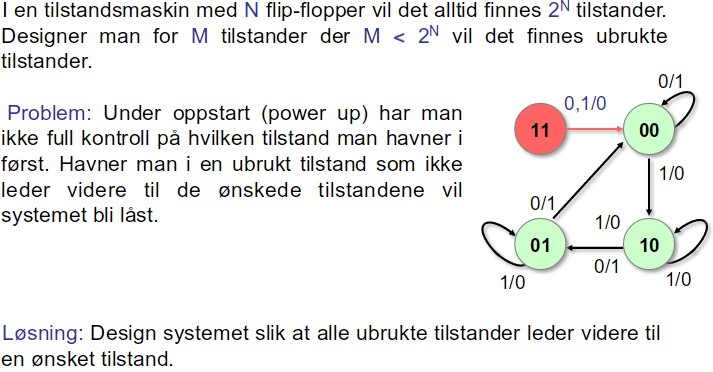
\includegraphics[scale = 0.6]{ubrukt.jpg}
		\caption{Ubrukte tilstander}
	\end{figure}
	
	\subsection{Designprosedyre(basert på D flip-floper)}
	\begin{figure}[H]
		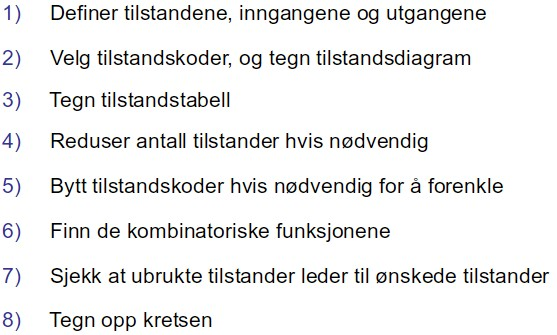
\includegraphics[scale = 0.6]{prosedyre.jpg}
		\caption{Designprosedyre}
	\end{figure}
	
	\subsection{Viktig for eksamen}
	Begreper besvarelsen må inneholde om omhandle for å kunne nå full poeng uttelling er: 
	
	Kunne bruke ord som handling og aksjon, tilstandstabell, tilstandsdiagram, tilstandskoder og tilordning av tilstand, input og output, relasjonen mellom flip - flop og antall tilstander, begrunnelse for valget av type flip - flop,	velge mer enn bare 2 tilstander, vise til kombinatorisk logikk for styringen av tilstandsmaskinen med input fra og til sensorer, implemenstasjon på portnivå, ubrukte tilstander, redusering av tilstander.
	
	\section{Datamaskinarkitektur}
	\subsection{Pipelining}
	
	Innfører samlebåndsprinsipp for eksekvering av instruksjoner
	
	Hver instruksjon må splittes opp i uavhengige deler(subinstruksjonener) som utføres etter hverandre
	
	Hver subinstruksjon kan utføres uavhengig av de andre subinstruksjonene 
	
	Neste instruksjon settes i gang før forrige instruksjon er helt ferdig.
	
	Hver instruksjon tar like lang tid å utføre, men prosessoren utfører flere instruksjoner i et gitt tidsrom. 
	
	En 4-trinns pipeline er den korteste som finnes for en CPU
	Men det å ha en 4-trinns pipeline betyr ikke at man får 4 ganger raskere prosessering. Det går alltid bort noe tid til administrering av instruksjoner.
	
	\subsubsection{ERROR 404 - Pipeline}
	
	Til enhver tid kan det være subinstruksjoner fra opptil 4 instruksjoner i en pipeline
	
	Noen ganger er ikke alle subinstruksjonene gyldige 
	
	Neste instruksjon kan ikke eksekveres rett etter hvis hopp-betingelsen slår til, noe som kalles HAZARD
	
	Det er tre typer HAZARD:
	
	-Resource Hazard
	
	-Data Hazard
	
	-Control Hazard
	
	
	\section{CMOS - Komplementær metalloksidhalvleder}
	
	\subsection{Transistor som bryter}
	\subsubsection{nMOS}
	En nMOS transistor har tre terminaler; Gate(inngang), Source og Drain. En nMOS transistor kan betraktes som en bryter, avhengig av inngang vil det kunne gå strøm mellom drain og source. Når inngangen er 0 går det ingen strøm mellom drain og source, og vi sier at transistoren er AV. Når inngangen er 1 kan det gå strøm mellom drain og source, og vi sier at transistoren er På.
	
	Lavest spenning - Source
	
	Høyest spenning - Drain
	
	En positiv strøm vil alltid gå fra drain til source.
	
	\subsubsection{pMOS}
	
	En pMOS transistor har også tre like terminaler akkurat som pMOS. Når inngangen er logisk 0 kan det gå strøm mellom source og drain, og vi sier at transisitoren er PÅ. Når inngangen er logisk 1 går det ingen strøm mellom source og drain, og vi sier at transistoren er AV.
	
	Høyest spenning - Source
	
	Lavest spenning - Drain
	
	En positiv strøm vil alltid gå fra source til drain.
	
	\subsubsection{pMOS + nMOS}
	
	Dersom vi setter en pMOS og en nMOS transistor sammen og kobler til spenningsreferansene Vdd og Vss får vi en CMOS inverter.
	
	CMOS teknologi er med andre ord grunnleggende inverterende.
	
	\begin{figure}[H]
		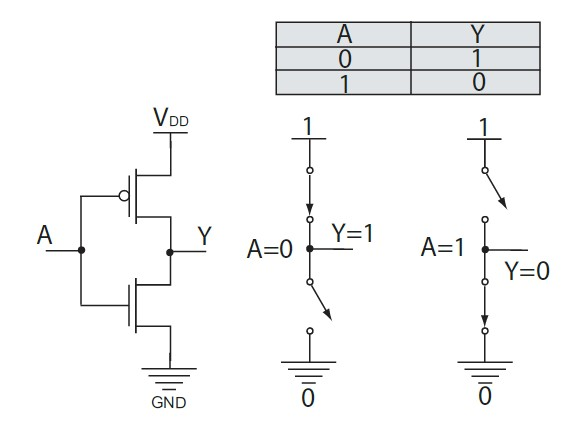
\includegraphics[scale = 0.6]{CMOSinv.jpg}
		\caption{Inverter skjematikk og sannhetstabell}
	\end{figure}
		
	\subsection{MOS transistorer}
	MOSFET - Metal On Semiconductor Field Effect Transistor - er integrerte transistorer.
	
	nMOS - fordi Source og Drain terminalene er koblet til n-type silisium.
	Disse områdene kalles for diffusjon og er kraftig dopet med et stort antall frie elektroner. Diffusjonsområdene ligger i en svakt dopet silisium halvleder som kalles substrat.Mellom gates og p-substrat er det et isolerende sjikt som separerer gaten fra substrat slik at det ikke skal gå strøm mellom gate og substrat.
	
	pMOS - fordi Source og Drain terminalene er koblet til p-type silisium. Disse områdenen kalles diffusjon og er kraftig dopet med et stort antall frie hull. Ved å sette på en positiv spenning(logisk 1) på gate terminalen vil elektroner tiltrekkes overfalten på halvlederen og invertere p-substrat til n-positiv substrat.
	
	\subsection{Fakta og regler}
	
	Det er vanlig i digital CMOS å benytte minimumsstørrelser på ulike strukturer, dette medfører et redusert arel og mindre tidsforsinkelse. Liten tidsforsinkelse gir raske kretser som kan fungere med svært høye klokkefrekvenser.
	
	Vi definerer opptrekksnettverk og nedtrekksnettverk som på dersom det finnes en strømvei mellom utgangen og spenningsreferesne, Vdd(1) og GND(0).
	
	Et nedtrekk er PÅ dersom det finnes en serie av nMOS transistorer som alle er PÅ og som forbinder utgangen med GND, i motsatt tilfelle er nedtrekk AV.
	
	For et opptrekk som er PÅ finnes det en serie av pMOS transistorer som alle er PÅ og som forbinder utgangen med Vdd, i motsatt tilfelle er opptrekket AV.
	
	I komplementær CMOS logikk vil alltid en og bare en av opptrekk- og nedtrekksnettverkee være på.
	
	AND = (*)
	NAND = $\overline{(*)}$
	
	OR = (+)
	NOR = $\overline{(+)}$
	
	\begin{figure}[H]
		\includegraphics[scale = 0.6]{OPPned.jpg}
		\caption{Generell logisk port med opptrekk bestående av pMOS transistorer og nedtrekk bestående av nMOS transistorer}
	\end{figure}
	
	\subsection{Serie og parallelkobling}
	nMOS i serie = NAND dersom GND = 0 på minst en inngang, $\overline{A*B}$
	
	\begin{figure}[H]
		\includegraphics[scale = 0.6]{nMOSserie.jpg}
		\caption{nMOS transistorer i serie}
	\end{figure}
	
	nMOS i parallell = NOR dersom Vdd = 1 på minst en inngang, $\overline{A+B}$
	
	\begin{figure}[H]
		\includegraphics[scale = 0.6]{pMOSpara.jpg}
		\caption{pMOS transistorer i parallellkobling}
	\end{figure}
	
	pMOS i serie = NOR dersom Vdd = 1 på minst en inngang,$\overline{A+B}$
	
	\begin{figure}[H]
		\includegraphics[scale = 0.6]{pMOSserie.jpg}
		\caption{pMOS transistorer i serie}
	\end{figure}
	
	pMOS i parallell = NAND dersom GND = 0 på minst en inngang, $\overline{A*B}$
	
	\begin{figure}[H]
		\includegraphics[scale = 0.6]{pMOSpara.jpg}
		\caption{pMOS transistorer i parallellkobling}
	\end{figure}
	
	\subsection{Komplementær logikk}
	
	Eks på en funksjon implementert ved CMOS
	$Y = \overline{(A \times B) + (C \times D)}$
	
	Nedtrekket vil bestå av nMOS transistorer og vi har at Y bare kan bli 0 når $(A \times B) + (C \times D) = 1$ Som forutsetter at A*B eller C*D er på. Nedtrekket må da bestå av to grener med seriekoblete nMOS transistorer.
	
	Opptrekket vi bestå av pMOS transistorer og vi har at Y bare kan bli 1 når $(A \times B) + (C \times D) = 0$ Som forutsetter at A og/eller B $(A \times B = 0)$ og C og/eller D $(C \times D = 0)$ er PÅ, altså 0. Opptrekket må da bestå av to grener med	parallellkoblete pMOS transistorer. Til slutt må disse to parallellgrenen settes i serie slik at forutsetningen for opptrekket blir oppflyt.
	
	\begin{figure}[H]
		\includegraphics[scale = 0.6]{CMOSeks.jpg}
		\caption{Komplementær CMOS port for funksjonen $Y = \overline{(A \times B)+(C \times D)}$}
	\end{figure}
	
	
	
\end{document}